\chapter{Work Experience} % Main chapter title

\label{Chapter2} % Change X to a consecutive number; for referencing this chapter elsewhere, use \ref{Chapter2}

\lhead{Chapter 2. \emph{Work Experience}} % Change X to a consecutive number; this is for the header on each page - perhaps a shortened title

I have had a total of six work placements since the start of my gap year.
Figure \ref{timeline} provides a timeline of the companies I have worked at.
The focus of this chapter will be on my placement at Sunamp, which was specifically done as part of my \textit{Industrial Project}.
After describing my experience at Sunamp, I will briefly describe my other work experiences.

\begin{figure}[htbp]
	\centering
	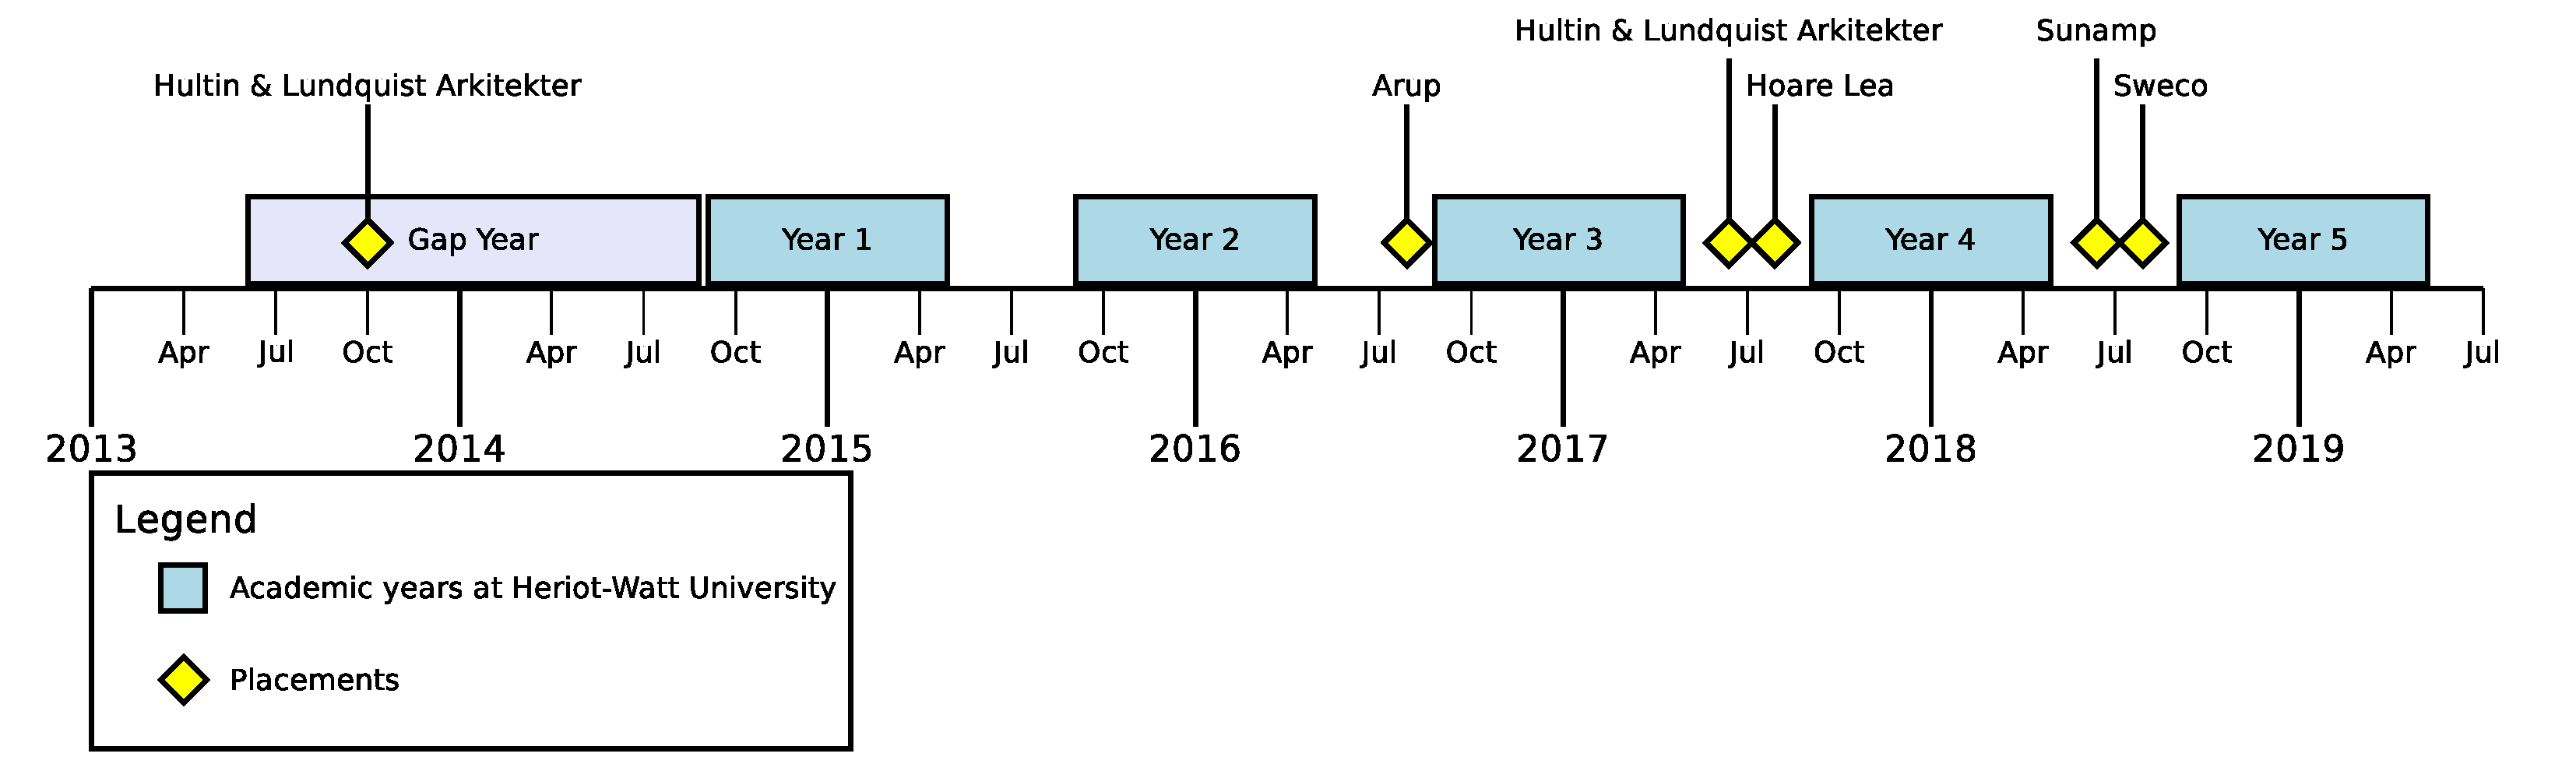
\includegraphics[width=\textwidth]{figures/IP-Timeline.eps}
	\rule{\textwidth}{0.5pt} % use line???
	\caption{Timeline of my work placements since my pre-university gap year.}
	\label{timeline}
\end{figure}


%----------------------------------------------------------------------------------------
%	SECTION 1
%----------------------------------------------------------------------------------------

\section{Sunamp, July - August 2018}

Sunamp is a newly established business that specialises in the research, production and sales of heat batteries that are based on phase change materials (PCMs).
The PCMs, developed and manufactured by Sunamp, are non-toxic, non-flammable, eco-friendly and patented in the UK and China, with patents pending in other countries \citep{SunampAutomotive}.
The PCMs operate at different temperatures, allowing the storage of heat (up to 1000$^{\circ}$C) or coolth (less than 0$^{\circ}$C) (see Figure \ref{pcm_temp_range}).
Currently, the company's main markets are buildings, where their heat batteries can be used for the production of hot water and space heating, and automobiles, where their heat batteries can be used for the refrigeration of transported goods.

\begin{figure}[htbp]
	\centering
	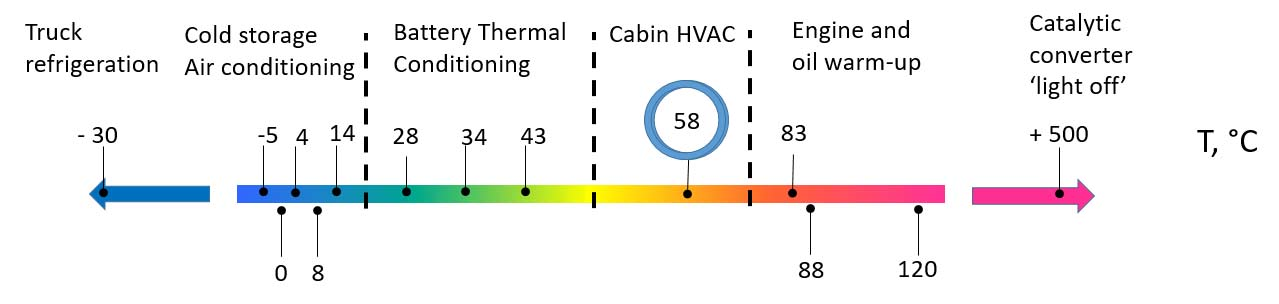
\includegraphics[width=\textwidth]{figures/temperature-range-of-PCMs.jpg}
	\rule{\textwidth}{0.5pt} % use line???
	\caption{The temperature range of Sunamp's PCMs in degrees Celsius \citep{SunampAutomotive}.}
	\label{pcm_temp_range}
\end{figure}

Sunamp was founded by Andrew Bissell (CEO) and is based in Macmerry, East Lothian.
They have a small office building, which features a workshop and chemistry laboratory on the ground floor and an open-plan office on the first floor, and a factory across the road where they have additional test facilities but primarily do large-scale manufacturing and packaging of heat batteries.
Around 20 people work in the office and five in the factory.


%-----------------------------------
%	SUBSECTION 1
%-----------------------------------

\subsection{Description of work experience}

My placement at Sunamp started on Tuesday 3\textsuperscript{rd} July 2018 and ended on Friday 10\textsuperscript{th} August 2018.
I worked a total of 198 hours there across six weeks, averaging at about 6.8 hours of work per day (see log in Appendix ... \hl{blur out sensitive info before adding to appendix}).
\hl{My purpose/ job description ...}
My time at Sunamp can roughly be divided up into two \hl{areas/ aspects}: learning about Sunamp's work and development, and producing work for Sunamp.


\subsubsection{Learning about Sunamp}

The majority of my first week at Sunamp consisted of my familiarisation with the company and their products.
The week started with an induction from Susan Lang-Bissell (MD) where we went over my contract, office information, health and safety regulations (amongst other things) and I got a brief tour of the factory.
The induction was followed by an introduction from Joan Pisanek, the Business Development Manager, to UniQ (Sunamp's latest range of heat batteries for buildings) and some of Sunamp's projects.
I used the rest of the week to familiarise myself with and try to understand their products by consulting Joan's PowerPoint presentations and the UniQ manuals,
% working through Joan's Buchlyvie project (\hl{see Appendix ...}), 
and attempting a UniQ Product Training Exercise developed by Sandy.

Santokh Gataora, \hl{colloquially known as} Sandy, is Sunamp's Technical Director.
He has a vast experience in building services engineering and helped develop the UniQ product range.
He writes and continues to refine the UniQ manuals as he guides the company in the engineering and application aspects of their UniQ heat batteries in buildings.
When I joined the company, UniQ was a very recent development that the sales team was still learning about.
The week I arrived at Sunamp, Sandy had sent out an exercise for the sales team to complete for the following week's UniQ Product Training Workshop.
The exercise instructions and my answer \hl{can be found in Appendix ... blur out people's names in email}.
I went on to attend the training workshop, where the sales team and I learned about the UniQ product range in greater depth and briefly went over the solution to the exercise.
\hl{Comment on my answer vs. solution?}

During my second and third weeks at Sunamp, I received more thorough tours of the factory, workshop and chemistry laboratory.
At the factory I got an understanding of the assembly of the heat batteries.
This broadly consists of the selection of a heat exchanger, the installation of the heat exchanger and pipes inside an insulated container, the sealing of the container, the mixing tank for the PCM, the pouring of the PCM into the container, and the cooling-off of the finalised heat battery for the next few days.
\hl{Sketch cross-section of heat battery! Am I allowed though?}

During the workshop and laboratory tour, I gained a deeper understanding of the making and performance of the PCMs and the selection of materials that go inside a heat battery.
Some of the things I learned are:
\begin{itemize}
    \item The high energy density of the PCMs is what allows Sunamp's heat batteries to be 2-4 times smaller than their equivalent hot water cylinders.
    \item Sunamp's chemists cycle and analyse PCM mixtures through solid-liquid and liquid-solid phase transitions to assess the stability of the mixtures' phase transitions over time. The more stable the transitions are, the more suitable they are to be used in heat batteries.
    \item The chemists also need to test their supplier's materials for impurities which can significantly degrade the performance of PCM mixtures.
    \item Different PCM mixtures can react differently to aluminium and copper, the main metals that heat exchangers are built from. Sunamp typically uses all-aluminium finned-tube heat exchangers, but they'll sometimes create a PCM which corrodes aluminium. In these cases they might need to consider using copper-based heat exchangers, which are more expensive but might work out cheaper in the long-run when compared to the capital and operational costs of the heat batteries' equivalent hot water cylinders.
    \item Working with cold, medium and high temperature ranges, the chemists need to ensure that the plastic material of the container which holds the PCM can tolerate that PCM's temperature range. Therefore Sunamp typically uses different materials for containers that carry cold and warm/ hot PCMs.
\end{itemize}

During my fourth and fifth weeks at Sunamp, I attended to two presentations.
The first was a summary of the research carried out by two chemistry students that had spent the past year working on their dissertations at Sunamp.
I gained some insight into the technical aspects of the development of PCMs and was impressed that one of the student's PCMs might soon become patented and used for refrigeration in vehicles.
Sandy gave the second presentation which was an overview of the new UniQ product range to the whole company.
I think this was especially insightful for the chemists and engineers who are specialised in their specific areas and might not always see how all of their work contributes to the end-product (heat batteries) and their application (heating space and water in buildings).

During my sixth (and final) week, I was part of the tour and planning of Sunamp's Experience Room.
This room is designed to look and feel like a home, with a kitchen-like decor and sink in one corner.
One of the purposes of this room, which was still under construction, is to showcase Sunamp's heat batteries to customers by comparing them to their large equivalents on the common marketplace (e.g. hot water cylinders) and by showing how they integrate into a building and its systems (e.g. heat pumps
and boilers).
The second purpose of this room is for workshops where one is trained how to install Sunamp's heat batteries.

Throughout my brief placement at Sunamp, there has been a sense of rapid development and expansion.
The company started out by manufacturing batteries inside a small workshop, which has now grown into a factory which is still evolving with the construction of new testing facilities and training/ marketing spaces.
The company continues to recruit more engineers and scientists.
It also seems like more customers are hearing about and taking interest in Sunamp's heat batteries, in the UK and abroad.

\hl{See notebook notes on how to demonstrate technical understanding.}



\subsubsection{Producing work for Sunamp} \label{sec:sunamp_work}

% Ohhhh come on! I gotta write! Just blow off some steam. It doesn't have to be all thought out and structured to begin with. Just keep the hand on the keyboard and type! As Moira says, "Be confident." :D

I joined Sunamp in the wake of the development of their new product range called UniQ.
UniQ had been developed by Sunamp's engineers, notably Sandy, and explained in a manual.
However, the manual was too large and technical for the sales team (headed by Joan) to understand, navigate and use to efficiently match customers with the most suitable UniQ products.
Therefore, \hl{my purpose at Sunamp was to bridge the gap between engineering and sales (see Figure ...}).
This was to be done by creating concise and user-friendly documentation that would introduce and explain the UniQ range to customers and even be used by the sales team as an aide-memoire.
This project mainly consisted of me presenting existing content in new ways and boiling down a lot of technical \hl{information/ features} into meaningful and useful information and benefits for customers.

I started working on my project during my second week at Sunamp and completed it during my last week.
From my log, I have deducted that I worked \hl{at least/ more than} 138 hours on this project, which accounts for 70\% of my time at Sunamp.
This includes the time I spent working autonomously, meetings, \hl{investigations}, and my final presentation.

I ended up creating a series of documents about UniQ, most of which can be seen in Figure \ref{funnel}.
The documents formed a hierarchy, from very generic information at the top to more specific information going down.
This funneling of information reflects the customer's journey, from the time they become aware of a product until they decide to purchase it.
\hlc[cyan]{
When I was preparing for my presentation, I discovered that my funnel resembles a marketing strategy/ concept called the marketing funnel.
This starts out by making customers aware of a product and then increasingly provides more specific information as a customer becomes more interested until they decide to purchase the product.}
\hlc[green]{On reflection...
This corroborated/ validated my use of the funnel.}
At the top of the funnel were documents that introduced and gave an overview of the UniQ product range.
These consisted of the Overview Sheet and UniQ Product Selection Quiz.
At the next level of the funnel were documents that provided specific information about the individual UniQ products; these were called the Product Information Sheets (PISs).
At the bottom of the funnel was a document that provided installation guidelines for the UniQ batteries.


\begin{figure}[htbp]
	\centering
	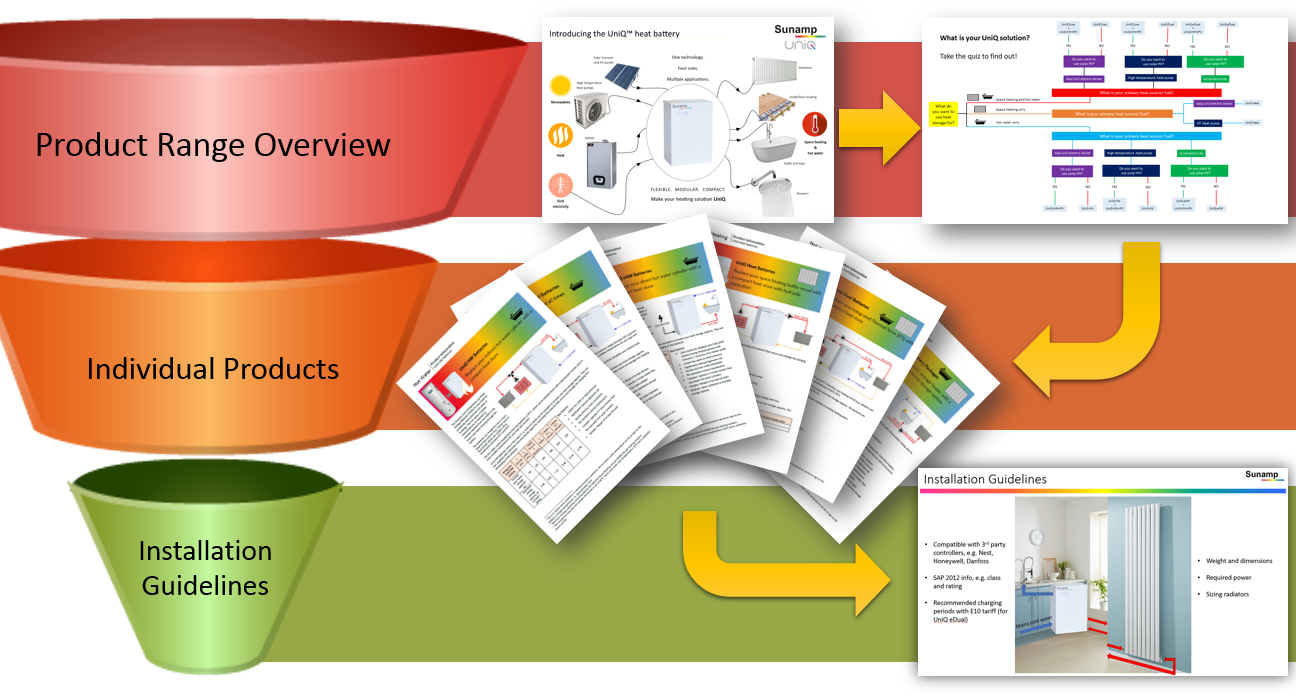
\includegraphics[width=\textwidth]{figures/Funnel.PNG}
	\rule{\textwidth}{0.5pt} % use line???
	\caption{The main outcomes of my UniQ project, ranked by a funnel-shaped hierarchy. \hl{Change title to Information Funnel or delete}}
	\label{funnel}
\end{figure}


Outside the heart of my project, embodied by the information funnel in Figure \ref{funnel}, I carried out a couple other tasks.
Among these was \hl{a document} I produced that contained additional information that was to be included in Sunamp's upcoming UniQ brochure.
Also, at the end of my placement, I gave a presentation to Sunamp's core staff, including the CEO, about my placement work.

The following sections will discuss my work in more detail.



\paragraph{UniQ Overview Sheet.}

I had not been asked to create a sheet that gave an overview of the UniQ product range.
I, however, thought it might be helpful to ease the customers' introduction to and understanding of UniQ.
The final Overview Sheet (see Appendix \ref{AppendixA}) introduces the UniQ battery by showing the possible inputs (renewables, heat and/ or electricity) and outputs (space heating and/ or hot water).
The battery is flexible when it comes to its inputs: these can range from boilers to heat pumps, and from grid electricity to PV panels.
Furthermore, the sheet features some catchy ways to describe UniQ, including the tag line ``Make your heating solution UniQ", that I came up with.
\hlc[green]{On reflection, the sheet misses the point of getting a heat battery. Why would I get a battery if I already have the means to generate space heating and hot water. I think this was raised during the meeting by Andrew and was to be rectified after I left.}

It turned out that Sunamp already had a diagram showing the inputs and outputs of a UniQ battery.
However, the staff expressed that they preferred mine for its clarity and visual impact.



\paragraph{UniQ Product Selection Quiz.} \label{sec:quiz}

As I was working on the PISs, the question of how a customer would know which UniQ product was most suitable to them \hl{loomed} in my mind.
``How will they even know which PIS to read?"
That is when I thought of creating a quiz in the form of a decision tree that would ask customers questions and guide them to the most suitable UniQ product for them based on their answers.
An added benefit of the quiz was that it would allow customers to explore the UniQ range easier and more informed, which would cut some of the sales team's initial \hl{customer-product match-making/ interface work}.

Figure \ref{quiz_draft} shows my first draft of the quiz.
I showed this to Joan when I pitched the quiz idea to her.
The idea was well received by her and Susan, so it escalated to another one of my sub-projects.
After creating a more polished second draft, I asked Sandy to give his expert feedback.
He responded with a re-arranged and more sophisticated decision tree.
This was the start of a process of iterations where I asked staff members for further feedback in order to refine the quiz design.
The final quiz can been seen in Appendix \ref{AppendixB}.


\begin{figure}[htbp]
	\centering
	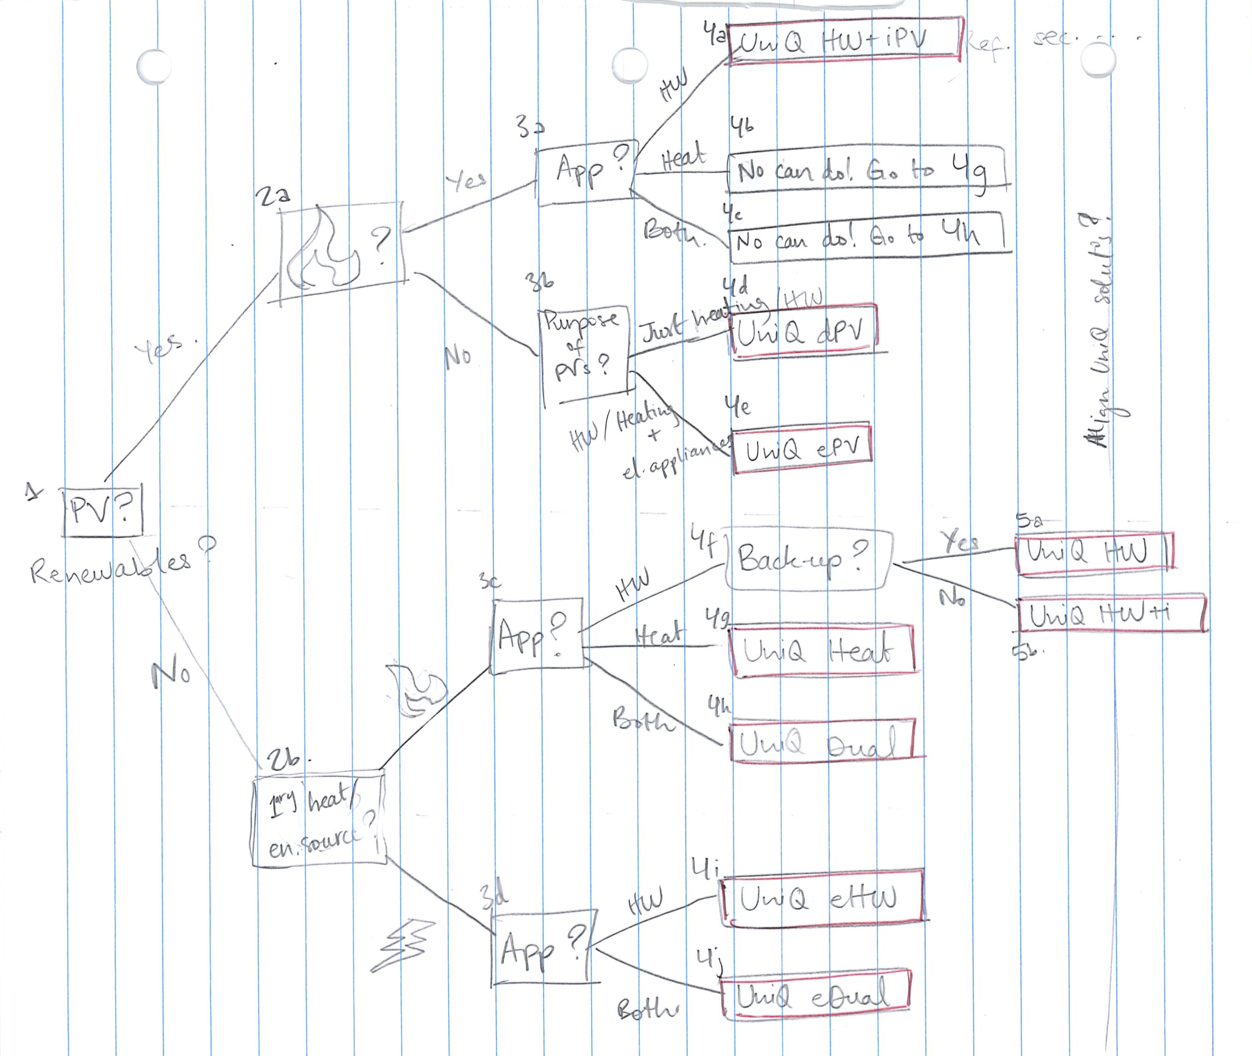
\includegraphics[width=0.5\textwidth]{figures/QuizSketch.png}
	\rule{\textwidth}{0.5pt} % use line???
	\caption{My first draft of the UniQ Product Selection Quiz.}
	\label{quiz_draft}
\end{figure}



\paragraph{UniQ Product Information Sheets (PISs).} \label{sec:piss}

Sandy asked me to produce a PIS for each of the UniQ products.
He gave me an outline of the type of information that would be included on each sheet, e.g. a brief description of the product and its operation, a diagram, and battery sizing information.
%, hydraulic connections, a wiring diagram, and a ``Do's and Don'ts!" list.
Every PIS was limited to two sides of an A4 page.

To accomplish this task, I used a variety of resources.
I obtained the relevant content from Sunamp's UniQ manuals and other documents.
Sometimes, however, the manuals were unclear or contradictory, e.g. regarding the dimensions of the UniQ batteries.
Therefore, to ensure accuracy of the PISs' content, I conducted little investigations e.g. measuring the dimensions of the UniQ batteries in the factory.
For the layout and presentation, I drew inspiration from a couple PISs by Mitsubishi (see one example in Figure \ref{mitsubishi}).
Similarly to the quiz, the production of the UniQ PISs was a process of iterations where I asked staff members (notably Joan and Sandy) for feedback throughout.
The creation of each UniQ PIS took around ten iterations or more.


\begin{figure}[htbp]
    \centering
        \begin{subfigure}{.48\textwidth}
          \centering
          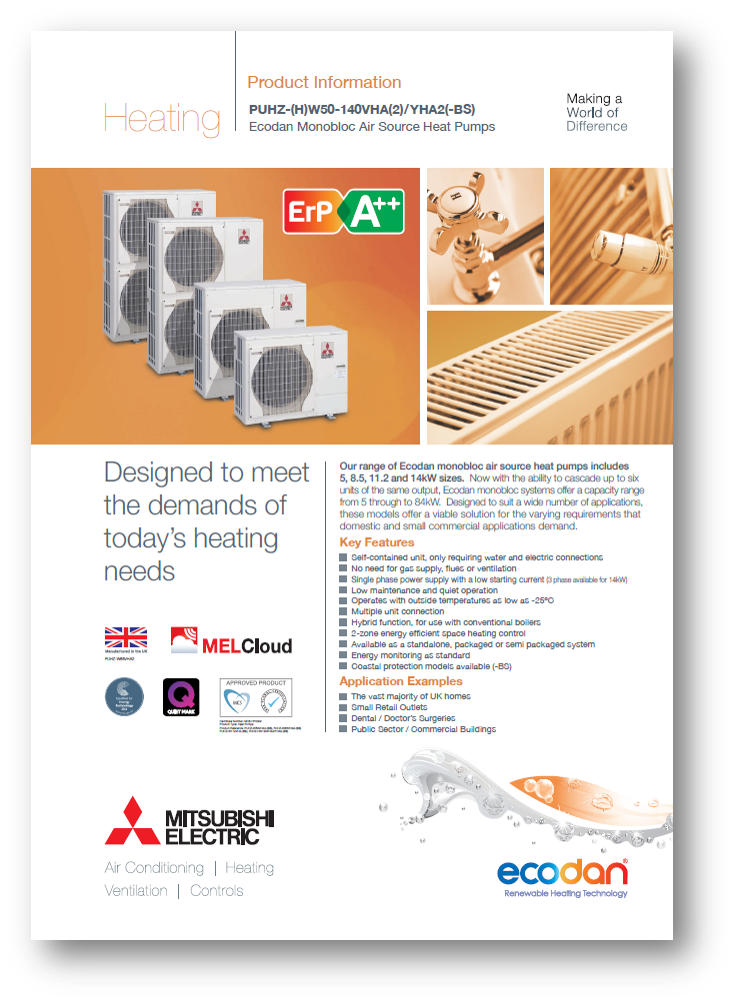
\includegraphics[width=\textwidth]{figures/Mitsubishi01.png}
%          \rule{\textwidth}{0.5pt} % use line???
          \caption{Front}
          \label{mitsubishi01}
        \end{subfigure}
        \begin{subfigure}{.485\textwidth}
          \centering
          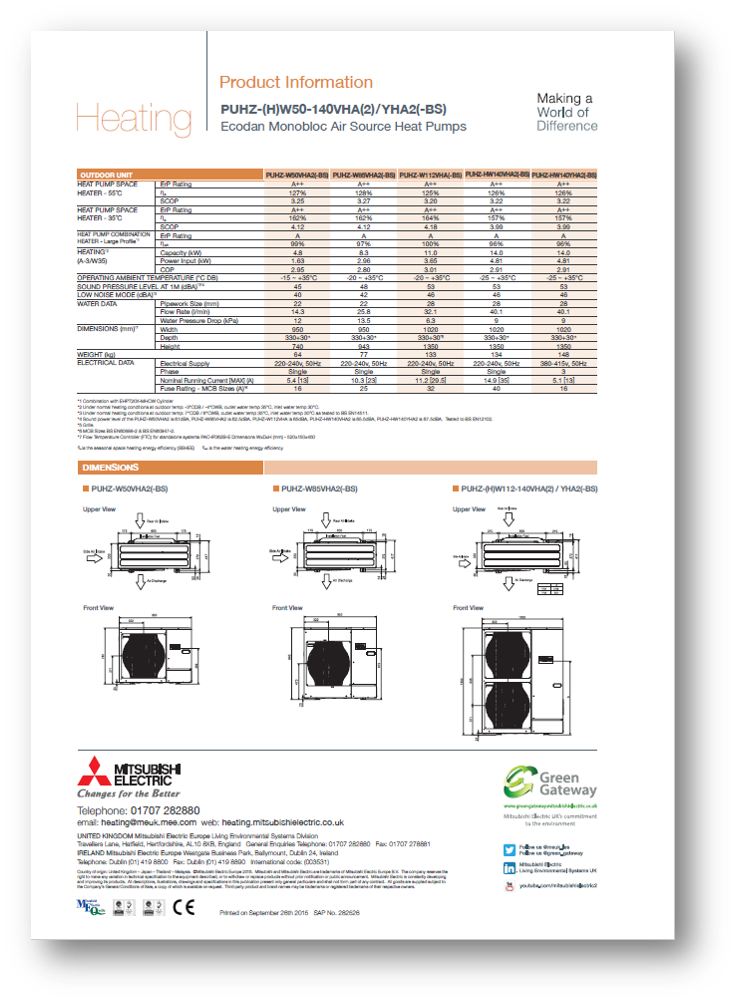
\includegraphics[width=\textwidth]{figures/Mitsubishi02.png}
%          \rule{\textwidth}{0.5pt} % use line???
          \caption{Back}
          \label{mitsubishi02}
        \end{subfigure}
    \rule{\textwidth}{0.5pt} % use line???
    \caption{One of Mitsubishi's PISs that I drew inspiration from \citep{ref:Mitsubishi}.}
    \label{mitsubishi}
\end{figure}


During my fifth week at Sunamp, I took part in a meeting with Susan, Joan, the Executive PA \hl{should I introduce abbreviations e.g. PA, CEO, PR and MD?} and a Public Relations (PR) Specialist that had come into the office to discuss the design of the UniQ brochure.
I presented drafts of the UniQ Overview Sheet, Product Selection Quiz and PISs to them.
This was a pivotal meeting as it was decided that my UniQ documents were going to be incorporated into the brochure and perhaps also be published on their website and as flyers.
Since a professional designer was going to polish the appearance of my work, I was asked to focus more on the content and its accuracy than the presentation.
That is why I have not included the UniQ logo in the PISs, for example.
% on finalising the content and ensuring its accuracy rather than worrying about the presentation.
% Also, other decisions were made, e.g. to remove the hydraulic connections and wiring diagrams.

Before the PISs could be sent to the PR Relations Specialist, they needed to be reviewed and approved by Sandy and, ultimately, Andrew.
By the end of my placement, however, I did not get the opportunity to run the last versions of the PISs by Andrew or Sandy.
In order to express my uncertainties of the latest drafts, I left the following message and amended the drafts accordingly:
\begin{itemize}
    \item ``\textcolor{red}{Texts in red} express my uncertainties in their expression or phrasing; these may require amending. This includes all the taglines.
    \item ``I have expressed other uncertainties in comments in the document markups."
\end{itemize}

The UniQ PIS drafts that I left with Sunamp can be found in Appendix \ref{AppendixC}.
\hl{Find a way to attach PISs.}
Figure \ref{breakdown} provides a breakdown of the PISs' structure and layout.


\begin{figure}[htbp]
    \centering
        \begin{subfigure}{\textwidth}
          \centering
          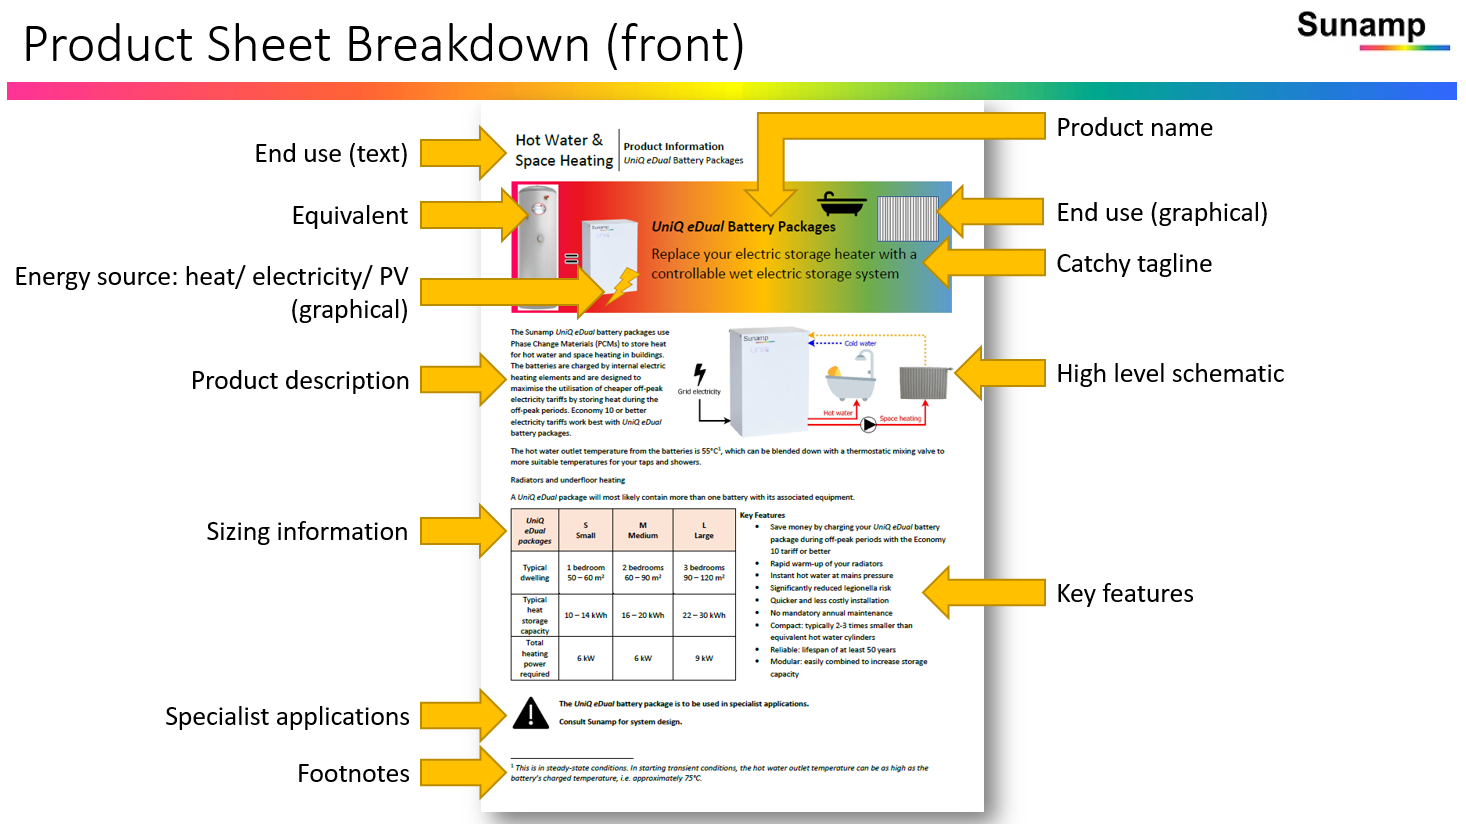
\includegraphics[width=\textwidth]{figures/PIS_breakdown_01.PNG}
%          \rule{\textwidth}{0.5pt} % use line???
%          \caption{Front}
          \label{breakdown01}
        \end{subfigure}
        \begin{subfigure}{\textwidth}
          \centering
          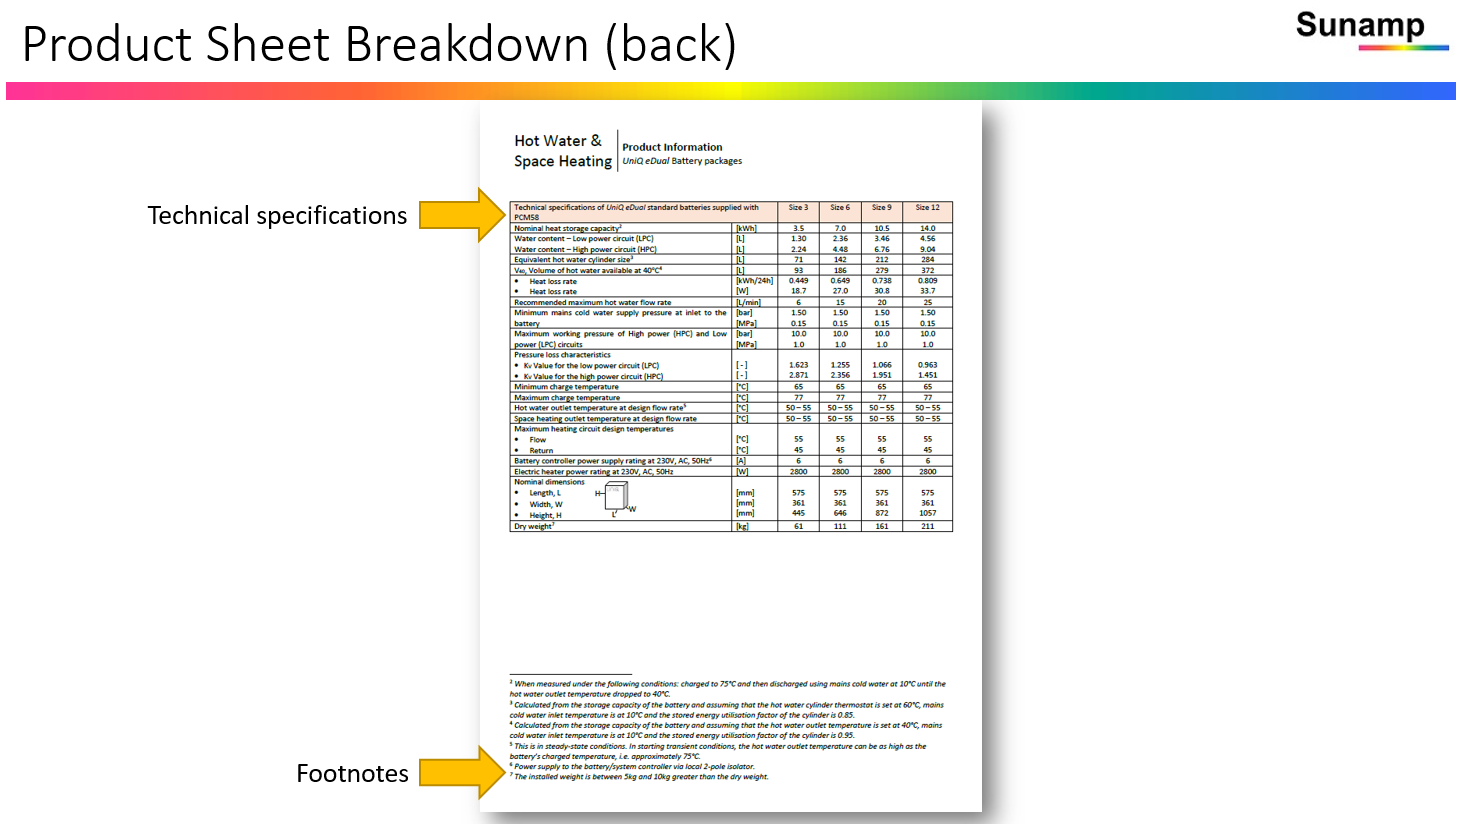
\includegraphics[width=\textwidth]{figures/PIS_breakdown_02.PNG}
%          \rule{\textwidth}{0.5pt} % use line???
%          \caption{Back}
          \label{breakdown01}
        \end{subfigure}
    \rule{\textwidth}{0.5pt} % use line???
    \caption{A breakdown of the composition of the UniQ PISs.}
    \label{breakdown}
\end{figure}



\paragraph{UniQ Installation \& Operation (I\&O) Sheets.}

Joan asked me to create documentation that presented important information that might affect the viability of using UniQ products in a system/ on a project, as well as answers to customers' frequently asked questions (FAQs).
``Will Sunamp install the UniQ battery for me?" and ``How will the UniQ battery integrate into my heating system?" are a couple FAQs, paraphrased.

The purpose of the I\&O Sheets was to provide customers with important information when they were considering or ready to purchase a UniQ battery.
Joan wanted me to include the answers to customers' frequently asked questions.

- Things customers need to know that might affect the viability of UniQ product implementation
- Currently just a vision… Lee…



\paragraph{Additional Information for UniQ Brochure.}



\paragraph{Presenting my Placement Work.}





%-----------------------------------
%	SUBSECTION 2
%-----------------------------------

\subsection{Analysis of/ Reflection on work experience}


%%%%%%%%%%%%%%%%%%%%%%%%%%%%%%%%%%%%%%%%%%%%%%%%%
\begin{comment}

\subsection{Application Process}

I learned about the opportunity of two paid placements with immediate start at Sunamp through David Campbell, the D11PJ course leader.
He had asked applicants for this placement to send him 100 words broadly describing their strengths and preferences, which he would then forward to Sunamp.
Hamish, a coursemate of mine, and I were both interested in this opportunity.
\hl{My hundred-word application went as follows:}

Strengths:
\begin{itemize}
	\item I am very familiar with the BIM process, having written a dissertation on collaboration with regards to BIM.
	\item I have work experience in mechanical and electrical consulting engineering.
	\item Organised, flexible, independent and cooperative.
\end{itemize}
Skills:
\begin{itemize}
	\item Advanced skills in Microsoft Office packages and Bluebeam Revu.
	\item Intermediate skills in LaTeX.
	\item Basic modelling skills in Revit, AutoCAD and IES-VE.
	\item Fluent in three languages (English, Swedish and French) with basic knowledge of Spanish.
\end{itemize}
Preferences/ interests:
\begin{itemize}
	\item Highly interested in learning about your application of Phase Change Materials in thermal storage batteries.
	\item Also interested in working with BIM and learning Bentley’s Hevacomp software packages.
\end{itemize}

After the applications, David introduced the two of us to Susan Lang-Bissell, the Managing Director (MD) of Sunamp, via email.
David asked us to liaise with Susan to arrange a meeting.
To do this, Hamish and I first established our availabilities in the upcoming days.
I then volunteered to liaise with Susan via email on our behalf to find a suitable date and time.

\hl{Try to be more reflective, and less descriptive.
Maybe record (vocally) the story, and then reflect on it out loud. THEN write about it.}

\end{comment}
